\documentclass[format=acmsmall, review=false]{acmart}


\usepackage{acm-ec-17}

\usepackage{booktabs} % For formal tables
\usepackage[ruled]{algorithm2e} % For algorithms
\graphicspath{ {experiments/} }
\usepackage{subcaption}

\renewcommand{\algorithmcfname}{ALGORITHM}
\SetAlFnt{\small}
\SetAlCapFnt{\small}
\SetAlCapNameFnt{\small}
\SetAlCapHSkip{0pt}
\IncMargin{-\parindent}

\usepackage{graphicx}     			% can better scale and rotate graphics than graphic package
\usepackage{multirow}               		% allows to have table cells on more than one row with "\multirow"
%\usepackage{amsmath, amsthm}	% !!! not for ACM template !!!
\usepackage{amssymb}                	% allows special symbols like "\nexists"
\usepackage{latexsym}               		% ? Dan
\usepackage{alltt}                  		% ? Dan
\usepackage{amsgen}                 	% ? Dan
\usepackage{amstext}               		% ? Dan
\usepackage{amscd}                  		% ? Dan
\usepackage{algorithmic}
\usepackage{url}
\usepackage{enumerate}
%\usepackage{cases}                  		% ? Dan
\usepackage{amsthm}
%\usepackage{mathtools}
%\usepackage{savesym}
\usepackage{amsmath}
\usepackage{tikz}
\usepackage{float}
\usepackage{enumitem}
\usepackage{mdwlist}
\usepackage{xspace}
\usetikzlibrary{arrows.meta}
\usetikzlibrary{fit,shapes,trees,shapes.geometric}
\usetikzlibrary{patterns,decorations.pathreplacing,calc}
\usetikzlibrary{arrows}
%\savesymbol{iint}
%\usepackage{txfonts}
%\restoresymbol{TXF}{iint}
\usepackage{bm}                     	% bold Greek letters
\usepackage{upgreek}              
\usepackage{xspace}    
\usepackage{color}              
\usepackage{colortbl}    
\usepackage{tabularx}
\usepackage{aliascnt}  	
\usepackage{mdframed}
\usepackage{caption}
\usepackage{makecell}
\usepackage{tcolorbox}
\usepackage{float}                 
\DeclareMathOperator*{\argmin}{\arg\!\min}
\usepackage{arydshln}
\setlength\dashlinedash{0.2pt}
\setlength\dashlinegap{1.5pt}
\setlength\arrayrulewidth{0.3pt}
\newcolumntype{L}[1]{>{\raggedright\let\newline\\\arraybackslash\hspace{0pt}}m{#1}}


\newcommand{\shaleen}[1]{{\color{blue} Shaleen: [{#1}]}}
\newcommand{\paris}[1]{{\color{SeaGreen} Paris: [{#1}]}}
\newcommand{\todo}[1]{{\color{red} ToDo: {#1}}}
\newcommand{\cull}[1]{{\color{red} [{#1}]}}
\newcommand{\introparagraph}[1]{\textbf{#1.}}   
\newcommand{\cut}[1]{}

\newenvironment{packed_item}{
\begin{itemize}
   \setlength{\itemsep}{1pt}
   \setlength{\parskip}{0pt}
   \setlength{\parsep}{0pt}
}
{\end{itemize}}

\newenvironment{packed_enum}{
\begin{enumerate}
   \setlength{\itemsep}{1pt}
  \setlength{\parskip}{0pt}
   \setlength{\parsep}{0pt}
}
{\end{enumerate}}

\newenvironment{packed_grep}{
\begin{description}
   \setlength{\itemsep}{1pt}
   \setlength{\parskip}{0pt}
   \setlength{\parsep}{0pt}
}
{\end{description}}
              
\newcommand{\ie}{{\em i.e.}\xspace}
\newcommand{\eg}{{\em e.g.}\xspace}
\newcommand{\ea}{{\em et al.}\xspace}
\newcommand{\aka}{{\em a.k.a.}\xspace}

\newcommand{\dtr}[0]{\twoheadrightarrow}     
 
\newcommand{\bQ}[0]{\mathbf{Q}}       
\newcommand{\bD}[0]{\mathbf{D}}       
\newcommand{\bR}[0]{\mathbf{R}}       
\newcommand{\bU}[0]{\mathbf{U}}     
\newcommand{\bT}[0]{\mathbf{T}}     
\newcommand{\bA}[0]{\mathbf{A}}     
\newcommand{\bB}[0]{\mathbf{B}}     
\newcommand{\bAp}[0]{\mathbf{A}}     
\newcommand{\bBp}[0]{\mathbf{B}}     
\newcommand{\bC}[0]{\mathbf{C}}     
\newcommand{\bV}[0]{\mathbf{V}}   
\newcommand{\bG}[0]{\mathbf{G}}     
 
\newcommand{\mS}[0]{\mathcal{S}} 
\newcommand{\mI}[0]{\mathcal{I}}   
\newcommand{\mF}[0]{\mathcal{F}}   
\newcommand{\mH}[0]{\mathcal{H}}   
\newcommand{\mE}[0]{\mathcal{E}}   
\newcommand{\mV}[0]{\mathcal{V}}   
\newcommand{\mC}[0]{\mathcal{C}}      
\newcommand{\mM}[0]{\mathcal{M}}   
\newcommand{\mL}[0]{\mathcal{L}}   
\newcommand{\mP}[0]{\mathcal{P}}   

\newcommand{\APS}[0]{\textsf{APS}}   
\newcommand{\DPS}[0]{\textsf{DPS}} 
\newcommand{\QPS}[0]{\textsf{QPS}} 

\newcommand{\agr}[2]{\mS_{#1}(#2)} 
\newcommand{\dagr}[2]{\overline{\mC}_{#1}(#2)} 
\newcommand{\setof}[2]{\{{#1}\mid{#2}\}}
\newcommand{\set}[1]{\{#1\}}   

\newcommand{\cmark}{\ding{51}}%
\newcommand{\xmark}{\ding{55}}%
\newcommand{\db}{\mathscr{D}}%
\newcommand{\upd}{\textsf{up}^\uparrow}

\newcommand{\ra}[1]{\renewcommand{\arraystretch}{#1}}

\definecolor{Gray}{gray}{0.9}
\definecolor{cardinal}{rgb}{0.77, 0.12, 0.23}
\definecolor{bondiblue}{rgb}{0.0, 0.58, 0.71}
\definecolor{babyblue}{rgb}{0.54, 0.81, 0.94}
\definecolor{lightgreen}{rgb}{0.67, 0.94, 0.82}
\definecolor{maize}{rgb}{0.98, 0.93, 0.37}

%\DeclareRobustCommand{\hlrone}[1]{{\sethlcolor{babyblue}\hl{#1}}}
%\DeclareRobustCommand{\hlrtwo}[1]{{\sethlcolor{maize}\hl{#1}}}
%\DeclareRobustCommand{\hlrthree}[1]{{\sethlcolor{lightgreen}\hl{#1}}}

\newcommand{\hlrone}[1]{{\color{black} {#1}}}
\newcommand{\hlrtwo}[1]{{\color{black} {#1}}}
\newcommand{\hlrthree}[1]{{\color{black} {#1}}}
\newcommand{\cmr}[1]{{\color{black} {#1}}}




\begin{document}
% Title portion. Note the short title for running heads 
\title[Revenue Maximizing Algorithms for Query Pricing]{Revenue Maximization for Query Pricing : Approximation Algorithms and Practical Advances}  



\begin{abstract}
In this paper we study the problem faced by a broker selling access to data with the goal of maximizing her revenue. The broker can set different prices for different queries made to the dataset, but must ensure that the pricing function does not provide the buyers with opportunities for arbitrage. This problem can be formulated as a revenue maximization problem with single-minded buyers and unlimited supply, for which several approximation algorithms are known. In this paper, we perform an extensive empirical evaluation of the performance of several pricing algorithms for the query pricing problem on real-world instances. In addition to previously known approximation algorithms, we propose several new heuristics and analyze them both theoretically and experimentally. Our experiments show that algorithms with the best theoretical bounds are not necessarily the best empirically. We identify algorithms and heuristics that are both fast and also provide consistently good performance when valuations are drawn randomly from a variety of distributions including zipfian, normal, and uniform distributions.
% In this paper, we present approximation algorithms for {\em query pricing} problem so as to maximize seller's revenue in the unlimited supply setting. We formulate the problem as an instance item pricing over {\em item hypergraph} where the buyers are {\em single minded} with subadditive valuations and investigate a variety of pricing strategies including {\em uniform item pricing} and {\em uniform bundle pricing}. \cite{guruswami2005profit} gave an $O(\log m + \log n)$ where $m$ is the number of customers and $n$ is the number of items with sum of all valuations as the upper bound. In our setting, we show that both item pricing and uniform bundle pricing exhibit a gap of $\Omega(m)$ from the optimal subadditive bundle pricing. Additionally, we investigate the revenue obtained using XOS pricing functions and show $O(\dots)$ approximation with a matching lower bound. We complement our theoretical results with extensive experiments on industry scale workloads. To this end, our experiments show that pricing algorithms behave very well in practice when valuations are drawn randomly from a variety of distributions including zipfian, normal and uniform distribution.
\end{abstract}


\maketitle

\section{Introduction}
\label{sec:intro}

The last decade or so has seen an explosion of data being collected from a variety of sources and across a broad range of areas. Many companies, including Bloomberg~\cite{bloomberg}, Twitter~\cite{twitterapi}, Lattice Data~\cite{lattice}, DataFinder~\cite{datafinder}, and Banjo~\cite{banjo} collect such data, which they then sell as structured (relational) datasets. 
These datasets are also often sold through online {\em data markets}, which are web platforms for buying and selling data: examples include BDEX~\cite{bdex}, Salesforce~\cite{salesforce} and QLik DataMarket~\cite{qlik}. Even though data sellers and data markets offer an abundance of data products, the pricing schemes currently used are very simplistic. In most cases, a data buyer has only one option, to buy the whole dataset (or a bundle of datasets) at a fixed price. Alternatively, the dataset is split into multiple disjoint chunks, and each chunk is sold at a separate price. 

However, data buyers are commonly interested in extracting specific information from a dataset and not in acquiring the whole dataset. Accessing this information can often be concisely captured through a {\em query}, or a sequence of queries. Selling the whole dataset at a fixed price forces the buyer to either pay more for the query than it is valued, or to choose not to access it. This means that valuable data is often not accessible to lay users, scientists, or entities with limited budgets, and moreover that data-selling companies and marketplaces behave suboptimally with respect to maximizing their revenue.

To address this problem, a recent line of research~\cite{KUBHS12,KUBHS13,deep2017qirana} in the database community introduced the framework of query-based pricing. A {\em query-based pricing scheme} tailors the purchase of the data to the user's needs, by assigning a price to each query issued over the dataset. Given a dataset $\db$ and a query $Q$ over the dataset, the user must pay a price $p(Q,\db)$ to obtain the answer $Q(\db)$ of the query. This price reflects only the value of the information learned by obtaining the query answer, and not the computational cost of executing the query. The work on query-based pricing has mainly focused on how to define a well-behaved pricing function, and how to develop system support for efficiently implementing a data marketplace.
In particular, a key property that a pricing function must obey is that of {\em arbitrage freeness}: it should not be possible for the buyer to acquire a query for a cheaper price through the combination of other query results. This is a type of incentive constraint. The arbitrage-freeness constraint makes the design of appropriate pricing functions a challenging task, especially since deciding whether a query is more informative than another query (or set of queries) is generally a computationally hard problem, and for practical applications it is critical that the price computation can be performed efficiently.

To overcome this computational barrier, \citet{deep2017qirana} proposed a setup where the seller and buyers have a common knowledge base $\mI$ consisting of multiple potential datasets. Each query (or set of queries) can then be thought of as a function that classifies datasets. The answer to a query identifies the collection of datasets in $\mI$ that are consistent with that answer. Whether a query is more informative than another then amounts to whether it identifies more inconsistent datasets than the latter. The benefit of this restricted model is that the query pricing can now be cast as a problem of pricing subsets over a ground set of items, each item being a dataset in the knowledge base $\mI$. The arbitrage-freeness constraint corresponds to the pricing function being monotone and subadditive. Of course, finding the optimal subadditive pricing is also a computationally hard problem. Furthermore, a general subadditive function, even if we manage to find one, can take exponential space to store. We therefore ask whether it is possible to find a simple pricing function that approximates the optimal subadditive pricing in terms of the seller's revenue. Observe that in the query pricing setting, there is no cost to the seller for replicating answers to queries, and so we can model the seller as having {\em unlimited supply} for each item. We further assume that buyers are single minded---each buyer wants to buy the answer to a single query.

% To overcome this computational barrier, one possible solution proposed in~\cite{deep2017qirana}  is to model each query $Q$ as a {\em bundle} of items $B(Q)$ from a common itemset $I$. Then, the arbitrage-free constraint translates to the requirement that the pricing function must be {\em monotone} and {\em subadditive} when viewed as a set function. Among such set functions, of particular practical interest are the additive and constant functions. An additive function gives to each item $i \in I$  a weight $w_i \geq 0$, and assigns the price $p(Q,\db) = \sum_{i \in B(Q)} w_i$, while a constant function simply assigns the same  price to every query, \ie $p(Q,\db) = p$.
% However, prior work has not answered the fundamental question of how one can choose among the possible set functions (or subclasses of them) the one that maximizes the revenue of the seller. 

Revenue maximization with unlimited supply and single-minded buyers has been studied extensively from a theoretical perspective and a number of approximation algorithms are known (see, e.g., \cite{guruswami2005profit,balcan2006approximation,briest2006single}). We discuss these algorithms in detail below. These algorithms produce pricings with worst case approximation factors logarithmic in one or more of the natural parameters of the instance, and these results are known to be tight to within constant factors in the worst case. But how well do these approximation results hold up in practice? Does the seller really need to give up on all but a logarithmic fraction of the optimal revenue in order to gain computational efficiency? Which of these algorithms should a practitioner use, and what features of the problem instance dictate this choice? These are some of the questions we study in this paper.


% This literature aims to obtain worst case approximation guarantees for revenue using additive pricing functions, a.k.a. item pricing. An item pricing gives to each item $i$  a weight $w_i \geq 0$, and assigns the price $p(S) = \sum_{i \in S} w_i$ to a bundle $S$ of items. There are a number of different algorithms and corresponding analyses in literature that produce item pricings with worst case approximation factors logarithmic in one or more of the natural parameters of the instance---the number of items $n$, the number of bundles $m$, the size of the largest bundle $k$, and the maximum number of bundles any item belongs to $B$. Many of these analyses are tight to within constant factors in the worst case.

\vspace{1em}
\noindent
{\em The goal of this work is to investigate how well theoretical performance bounds for revenue maximization with unlimited supply hold up in practice, using the setting of query pricing for data markets as an application.} 
\vspace{1em}

We perform an experimental study to evaluate the quality of various pricing algorithms for different problem instances, both synthetic and real. The approximation ratio of a pricing algorithm is just one of many features that determine how practical the algorithm is. We compare algorithms in terms of the revenue obtained, as well as their running time and the representation complexity of the pricing produced. Enroute we develop a new algorithm and a post-processing heuristic to use in conjunction with known algorithms to improve performance, and prove some new performance bounds. We now discuss these contributions in more detail.

We study three kinds of pricings. The first, {\em uniform bundle pricing}, assigns the same price to every bundle and is the default pricing scheme in many data markets currently. The second, additive or {\em item pricing}, assigns a price to each item and charges a price for each bundle equal to the sum of prices for the items in the bundle. Most approximation results known produce item pricings. Third, we consider a much more general class of pricings, namely {\em XOS or fractionally subadditive pricings}. These pricings are much more expressive than item or uniform bundle pricings, while at the same time having small representation size. We show that XOS pricings can achieve a logarithmic factor larger revenue than the better of the latter two. However, there are no algorithms known to exploit the benefits of this class of pricings.

We study the performance of the following pricing algorithms. In quantifying performance, several parameters of the instance are relevant: the number of items $n$, the number of bundles $m$, the size of the largest bundle $k$, and the maximum number of bundles any item belongs to $B$. In the query pricing setting it is usually the case that $B\le m\ll k\le n$, so algorithms with approximation factors and running time depending on $B$ or $m$ are generally better than those depending on $k$ or $n$.
\begin{itemize}
\item {\bf Capacity-based item pricing.} This algorithm due to Cheung and Swamy~\cite{cheung2008approximation} achieves the best known worst case approximation ratio for revenue, namely $O(\log B)$. This ratio is tight. The algorithm involves solving multiple linear programs, each with $O(n)$ variables and constraints, for each instance of the problem and is therefore slow in practice.
\item {\bf Uniform item pricing.} This simple algorithm prices every item at the same amount, and achieves an approximation ratio of $O(\log n+\log m)$. 
\item {\bf LP-based post processing.} Given any item pricing, and the subset of bundles that get purchased by the corresponding buyers at those prices, we can ask whether it is possible to increase prices while selling the same bundles so as to extract more revenue. This optimization can be expressed as a linear program and solved efficiently. We apply this optimization as a post processing step to the above two algorithms achieving significant performance gains in experiments, although it does not improve the worst case approximation ratio.
\item {\bf Layering-based item pricing.} We develop a new greedy algorithm that partitions bundles into groups, each of which can be priced optimally to extract their entire value as revenue. We show that this algorithm achieves an $O(B)$ approximation in the worst case. Although this approximation factor is exponentially worse than that of the first algorithm, we observe that for many workloads the two algorithms achieve similar performance, and the simplicity and speed of the greedy algorithm gives it a distinct advantage. 
\item {\bf Uniform bundle pricing.} Finally, For the sake of comparison, we also implement and report results for the best uniform bundle pricing, namely one that assigns the same price to every bundle.
\end{itemize}


% We study the performance of three different pricing algorithms in this paper. The first is an item pricing algorithm due to Cheung and Swamy~\cite{cheung2008approximation} that achieves the best known worst case approximation ratio for revenue, namely $O(\log B)$. This algorithm involves solving multiple linear programs for each instance of the problem, and is therefore very slow in practice. The second algorithm we consider is an item pricing with a worse approximation ratio of $O(\log n+\log m)$. This is a simple algorithm that produces a uniform item pricing, namely one where all item weights, $w_i$, are equal. The simplicity of the algorithm allows for algorithmic improvements that do not hurt its approximation ratio but for some instances can greatly improve performance. We describe one such improvement in Section~\ref{section-approxalgo}. The third algorithm we study is an extremely fast greedy item pricing algorithm. We show in Section~\ref{section-approxalgo} that the greedy algorithm achieves a worst case approximation factor of $O(B)$. Although this approximation factor is exponentially worse than that of the first algorithm, we observe that for many workloads the two algorithms achieve similar performance, and the simplicity and speed of the greedy algorithm gives it a distinct advantage. For the sake of comparison, we also implement and report results for a constant pricing function, namely one that assigns the same price to every bundle (query). \todo{Say something about XOS?}

Our experimental study shows that the worst-case analysis of pricing algorithms does not capture how well the algorithms behave in real-world instances in terms of approximating the optimal revenue, for the specific application of query-based pricing. In particular, we observe that the structure of the bundles induced by different query workloads heavily influences the quality of approximation. For example, despite achieving the best known worst case approximation ratio, capacity-based item pricing did not achieve the best performance of the algorithms we tested in even one of our experimental setups. Our work suggests that a promising direction is to attempt to obtain better approximation guarantees by taking into account the structure of the bundles, and also the type of valuations that occur in real-world settings.

% In this paper, we tackle the above question building on ideas from the optimal pricing 
% literature~\cite{guruswami2005profit}. We consider the {\em unlimited supply} setting, where the 
% seller can sell any number of units of each query. This is a natural assumption in the context of a data market,
% since multiple buyers can request and purchase the same query.
% Additionally, we assume that the buyers are {\em single-minded}, so each
% buyer is interested in buying only a single query $Q$ (so a single bundle) for a price of $v_Q$; the buyer will
% purchase the query only if the price $p(Q, \db)$ does not exceed $v_Q$. We focus on the aforementioned two
% types of pricing functions that either assign a uniform price to every query, or perform item pricing. 
% In the case of item pricing, the problem of computing the revenue-maximizing prices can be cast as
% the well-studied {\em hypergraph vertex pricing} problem, where only approximation guarantees are known.











%
\section{Notation and Preliminaries}

We assume that there are $m$ customers (hyperedges) and $n$ items. Since we are in the {\em unlimited supply setting}, the seller has zero marginal cost  for each item, i.e, the seller can sell any number of units of each item. Additionally, the buyers are  {\em single minded}, which means that each customer is interested in buying only a single set of items corresponding to the hyperedge $e$ for price $v_e$. Buyers will purchase $e$ only if the price assigned to bundle $e$ is at most $v_e$. We will use $p^{b}_e$ and $p^{i}_e$ to denote the bundle and item prices respectively assigned by the algorithm. 
\section{The Query-Based Pricing Framework}
\label{sec:framework}


\textbf{\textit{Question 1.}} Given $m$ customers (hyperedges) and their valuations $v_i$, what is the revenue gap between the optimal arbitrage free pricing and: $(i)$ item pricing $(ii)$ uniform bundle pricing, using the pricing function $p^{a}(Q,\mathcal{D})$.

\vspace{1em}
We show that the gap is $\Omega(m)$ for uniform bundle pricing and this is tight. For item pricing, we show that gap is $\Omega(m)$. Given these results, it is tantalizing to wonder whether XOS pricing functions (rather than single additive function) helps bridge the revenue gap. 

\vspace{1em}
\textbf{\textit{Question 2.}} Given $m$ customers (hyperedges) and their valuations $v_i$, what is the revenue gap between the optimal arbitrage free pricing and XOS pricing function.

\vspace{1em}
Our main result for the second question is 

\section{Uniform Bundle and Item Pricing}

In this section, we present a brief discussion for worst-case guarantees on how well uniform bundle pricing and item pricing can approximate the 
optimal subadditive and monotone bundle pricing. Figure~\ref{fig:summary} summarizes the upper and lower bounds that are either known,
or we obtain in this paper.


\begin{figure}[t]
	\scalebox{.95}{
		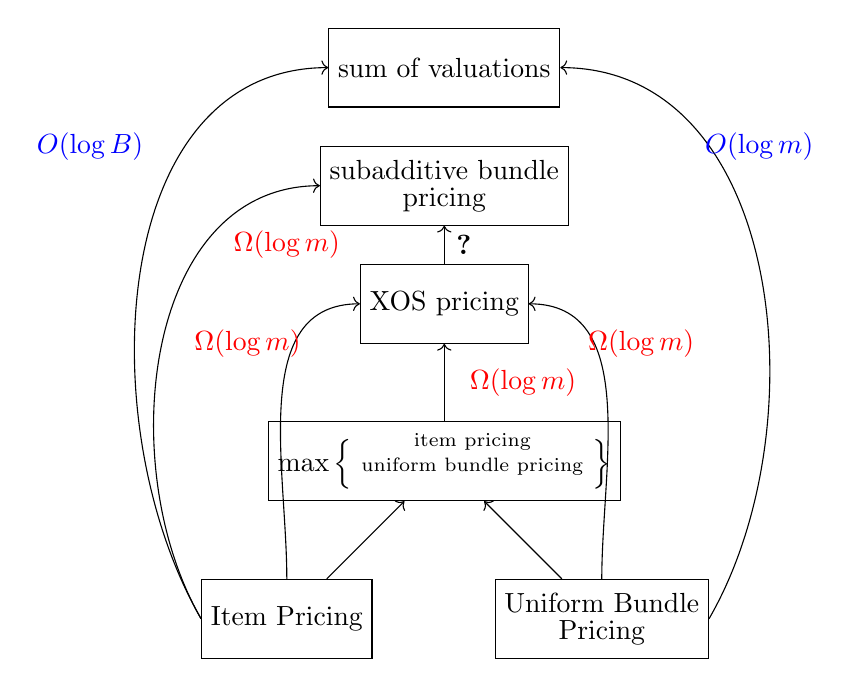
\begin{tikzpicture}
		\node (rectsum) [rectangle, draw, minimum width=7mm, minimum height=10mm] at (0,1.5) {sum of valuations};
		
		\node (rectbundle) [rectangle, draw, minimum width=7mm, minimum height=10mm] at (0,0) {\shortstack{subadditive bundle \\ pricing}};
		
		\node (rectxos) [rectangle, draw, minimum width=7mm, minimum height=10mm] at (0,-1.5) {XOS pricing};
		
		\node (rectmax) [rectangle, draw, minimum width=7mm, minimum height=10mm] at (0,-3.5) {$\max \Big\{$  \shortstack{\scriptsize item pricing \\ \scriptsize uniform bundle pricing} $\Big\}$};
		
		\node (rectitem) [rectangle, draw, minimum width=7mm, minimum height=10mm] at (-2,-5.5) {Item Pricing};
		
		\node (rectubundle) [rectangle, draw, minimum width=7mm, minimum height=10mm] at (2,-5.5) {\shortstack{Uniform Bundle \\ Pricing}};
		
		\draw [->] (rectubundle.east) to [out=60, in = 0] (rectsum);
		\node at (4,0.5) {\textcolor{blue}{$O( \log m)$}};
		\draw [->] (rectubundle) to [out=90, in = 0] (rectxos);
		\node at (2.5,-2) {\textcolor{red}{$\Omega( \log m)$}};
		\draw [->] (rectitem.west) to [out=120, in = -180] (rectsum.west);
		\node at (-4.5,0.5) {\textcolor{blue}{$O( \log B)$}};
		\draw [->] (rectitem) to [out=90, in = -180] (rectxos.west);
		\node at (-2.5,-2) {\textcolor{red}{$\Omega( \log m)$}};
		\draw [->] (rectxos) to  (rectbundle);
		\node at (0.25,-0.75) {\textbf{?}};
		\draw [->] (rectitem.west) [out = 120, in = -180] to  (rectbundle.west);
		\draw [->] (rectmax)  to  (rectxos);
		\draw [->] (rectitem)  to  (rectmax);
		\draw [->] (rectubundle)  to  (rectmax);		
		\node at (-2,-0.75) {\textcolor{red}{$\Omega( \log m)$}};
		\node at (1,-2.5) {\textcolor{red}{$\Omega( \log m)$}};
		
		\end{tikzpicture}
	}
	\caption{Results Summary: Red font show results in this paper; blue font shows existing known results}
	\label{fig:summary}
\end{figure}

\paragraph{Upper Bounds.}
It is a folklore result that for any hypergraph $\mH = (\mV, \mE)$ with valuations $\{v_e\}_{e \in \mE}$, one can always construct a uniform bundle price that is $O(\log m)$ away from
the sum of valuations $\sum_e v_e$, which is an upper bound on the optimal subadditive and monotone bundle pricing (for completeness, we provide a proof in Appendix~\ref{sec:appendix}). Similarly, we know from~\cite{cheung2008approximation} that item pricing can achieve a $O(\log B)$ approximation of the sum of valuations. Recall that 
$B$ is the maximum number of hyperedges that any vertex can be contained in, and hence $B \leq m$. 

\paragraph{Lower Bounds.}
Not surprisingly, the upper bound of $O(\log m)$ is tight in the worst case for both uniform item pricing and bundle pricing. In particular, we show the following stronger results:
%
\begin{enumerate}
\item There exists a hypergraph instance with additive valuations where any uniform bundle price produces revenue that is $\Omega(\log m)$ away from the optimal (Lemma~\ref{lem:lb1} in the appendix).
\item There exists a hypergraph instance with uniform valuations (\ie, each buyer has the same valuation for any hyperedge) where any item pricing produces revenue that is $\Omega(\log m)$ away from the optimal (Lemma~\ref{lem:lb2} in the appendix).
\item There exists a hypergraph instance with submodular valuations where any item pricing {\em and} any uniform bundle pricing is  $\Omega(\log m)$ away from the optimal (Lemma~\ref{lem:lb3} in the appendix).
\end{enumerate} 

The above lower bounds tell us that there are problem instances where uniform bundle pricing will be optimal, but item pricing will behave poorly, and vice versa. Moreover, there are instances where both subclasses of pricing functions will not perform well with respect to a submodular monotone function (which is a subset of subadditive and monotone bundle pricing).
 A straightforward corollary of the lower bound of Lemma~\ref{lem:lb3} is that even an XOS pricing function that combines a constant number $k$ of item pricing functions suffers from the 
 $\Omega(\log m)$ revenue gap. An open question that remains is whether an XOS pricing with larger $k$ can obtain a better approximation guarantee with respect to the optimal subadditive and monotone bundle pricing.




\section{Experimental Evaluation}

In this section, we will empirically evaluate the performance of known approximation algorithms for item pricing and bundle pricing. Our goal is to understand the behavior of the algorithms on practical \texttt{SQL} queries over real world datasets as well as the behavior on random hypergaphs. We will first describe our experimental setup, followed by the various knobs that we can control to create different instances of the hypergraph instances and valuations. 

\subsection{Experimental setup}

We perform all our experiments on $2.2$ GHz processor machine with $4$ cores and $16$ GB main memory running OS X $10.10.5$. \texttt{MySQL} is used as the underlying database for query processing and evaluation . Our implementation is written in \textsc{Python} as an enhancement in \textsc{Qirana} prototype system. \textsc{Qirana} generates random neighbors of a database as its support set over which query pricing is performed. The advantage of using neighbors is that we can succinctly represent the neighbor without storing the new database, i.e, we can represent the neighbor by storing only the \emph{update query} that generates the neighboring database. Thus, given a query $\bQ$ and support set $\mS$ for database $\db$, \textsc{Qirana} will compute the conflict set of the query. Then, the system will assign prices to each item in the conflict set.
Table~\ref{table:experiments} shows the experimental design space we consider. Our experiments will be over three different datasets. For each dataset and valuation model (which in turn will use different distributions), we compute the revenue that can be extracted using the algorithms listed. In order to compare different algorithms we use two upper bounds: $(i)$ sum of valuations, and $(ii)$ an upper bound on the optimal subadditive valuation. We find an upper bound on the optimal subadditive valuations by computing a linear program whose constraints encode the arbitrage constraints. Since the number of constraints can be exponential in the number of hyperedges, we optimize by greedily adding constraints for bundles with largest valuations and finding a set of bundles that cover the hyperedge with small valuations. As we will see later, this helps us compare the performance of algorithms with respect to the subadditive bound that can be better than sum of valuations. In all our experiments, we report each data point as an average over $5$ runs where we discard the first run to minimize cache latency effects.

\begin{table*} \centering
	\def\arraystretch{1.35}%
	\begin{tabular}{c|c|c|c}
		\toprule
		\textbf{Dataset} & \textbf{Algorithms} & \textbf{Workload} & \textbf{Valuation Model}\\ \midrule
		$\texttt{\bfseries world}$ dataset & \ubp & SQL query workload & Sampled Bundle Valuations \\ 
		& \uip & Random workload & Scaled Bundle Valuations \\ 
		& \lpip &  & Additive Bundle Valuations \\ 
		& \cip & &  \\
		& layering &  &  \\
		\bottomrule
	\end{tabular}
	\caption{Experimental Design Space}
	\label{table:experiments}
\end{table*}

\subsection{Workload and Dataset Characteristics}

\begin{figure}[!h]
	
	\begin{minipage}[t]{0.49\linewidth}
		\centering
		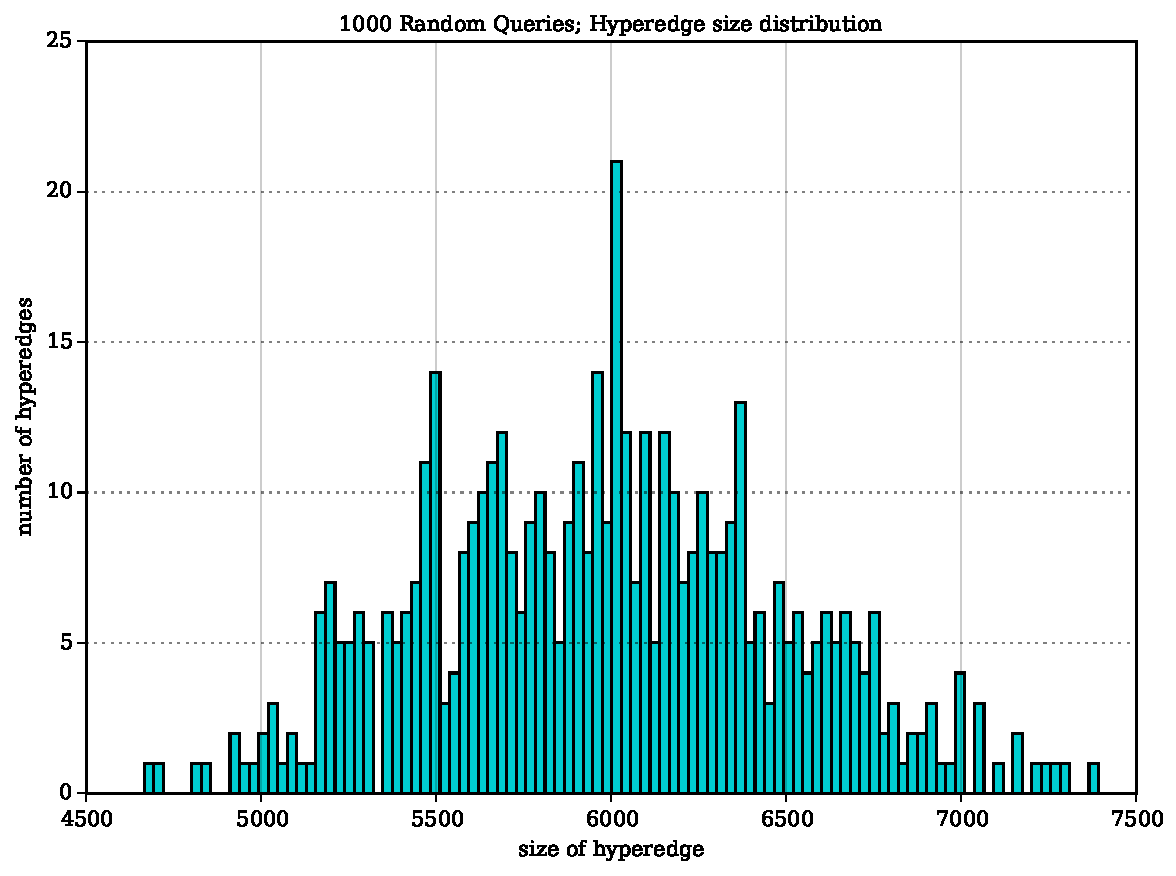
\includegraphics[scale=0.35]{histogramhyperedgesizerandomworkload.pdf}
		\caption{Random workload} \label{fig:histogramrandom}
	\end{minipage}
	\begin{minipage}[t]{0.47\linewidth} 
		\centering
		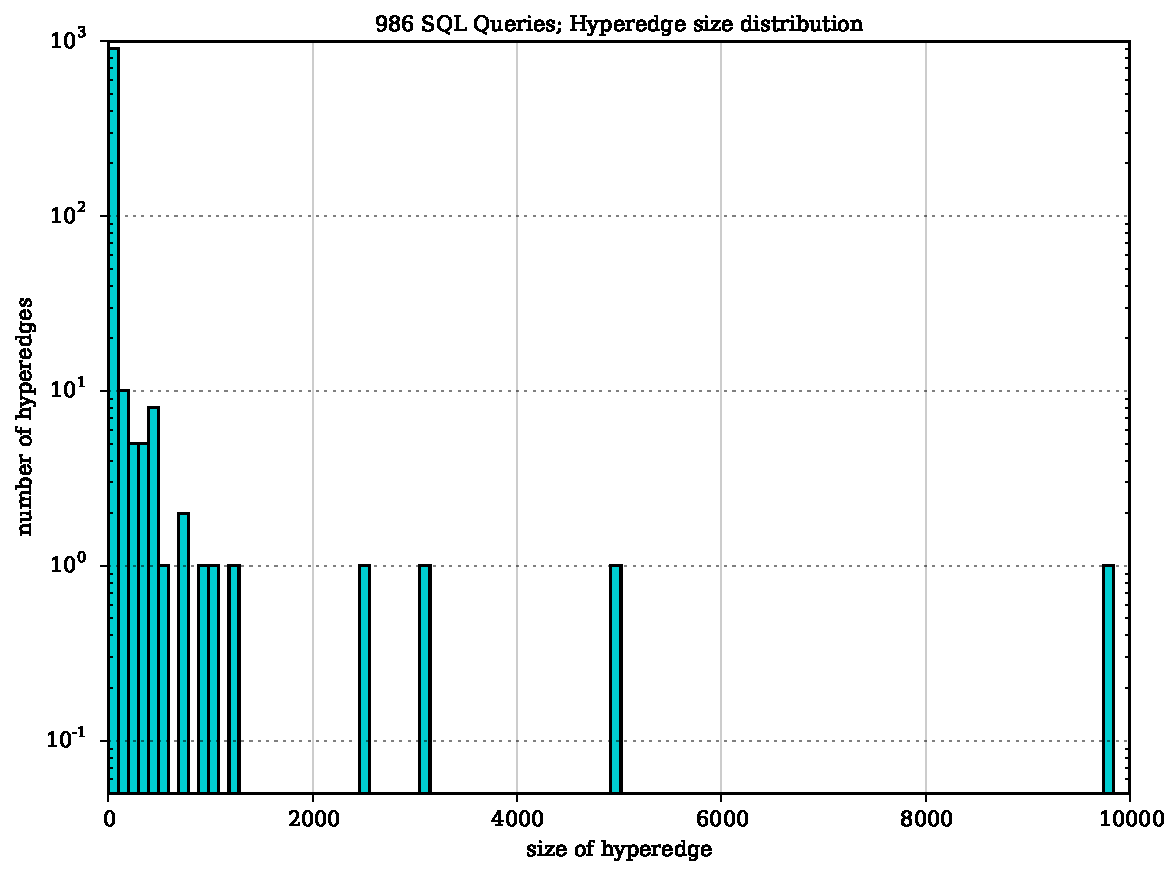
\includegraphics[scale=0.35]{histogramsqlworkload.pdf}
		\caption{SQL workload} \label{fig:histogramrealqueries}
	\end{minipage}        
\end{figure}  

\begin{table*}[] \centering
	%\ra{1.3}
	\begin{small}
		\begin{tabular}{@{}lrrr@{}}\toprule
			\textbf{Workload} & \textbf{\# Queries} & \textbf{Maximum Item Degree} & \textbf{Average edge size} \\ \midrule
			
			\textbf{SQL Queries} &  986 & 22 & 5982.07  \\ \hdashline
			\textbf{Random Queries} &  1000 & 400 &  41.67  \\
			\bottomrule
		\end{tabular}
	\end{small}
	\caption{Workload Characteristics}
	\label{table:workload:characteristics}
\end{table*}

We will now describe briefly the characteristics of the workload and datasets used. The first dataset we use is the $\texttt{\bfseries world}$ dataset, a popular database provided for software developers. 
It consists of $3$ relations: $\texttt{\bfseries Country}$,$\texttt{\bfseries CountryLanguage}$ and $\texttt{\bfseries City}$ which contain $5000$ tuples and $21$ attributes. We construct a support set of size $15000$ by randomly choosing neighboring databases. 
The query workload consists of $986$ queries containing selection, projections and join queries with aggregations. We construct the workload by generating changing the predicates in queries. The full list queries in this dataset is present in the appendix.

The second workload also uses $\texttt{\bfseries world}$ dataset but consists of randomly chosen selection and projection queries. To generate a random selection query, we  sample without replacement a subset of primary keys that will included in the query. Similarly, for projection queries, we choose a subset of attributes that will form the projection list of the query.

Figure~\ref{fig:histogramrandom} and~\ref{fig:histogramrealqueries} depicts the distribution of the hyperedge size distribution for both the workloads. Throughout our experiments, unless specified otherwise, the hypergraphs remain fixed.


\subsection{Experiment Results for SQL Workload}

Our first set of experiments is to understand how the approximation algorithms behave on real world queries. 


\subsubsection{Sampling Bundle Valuations} 
In this part of the experiment, we will sample valuations for the bundles from a fixed distribution.

\begin{figure}[!t]
	\centering
	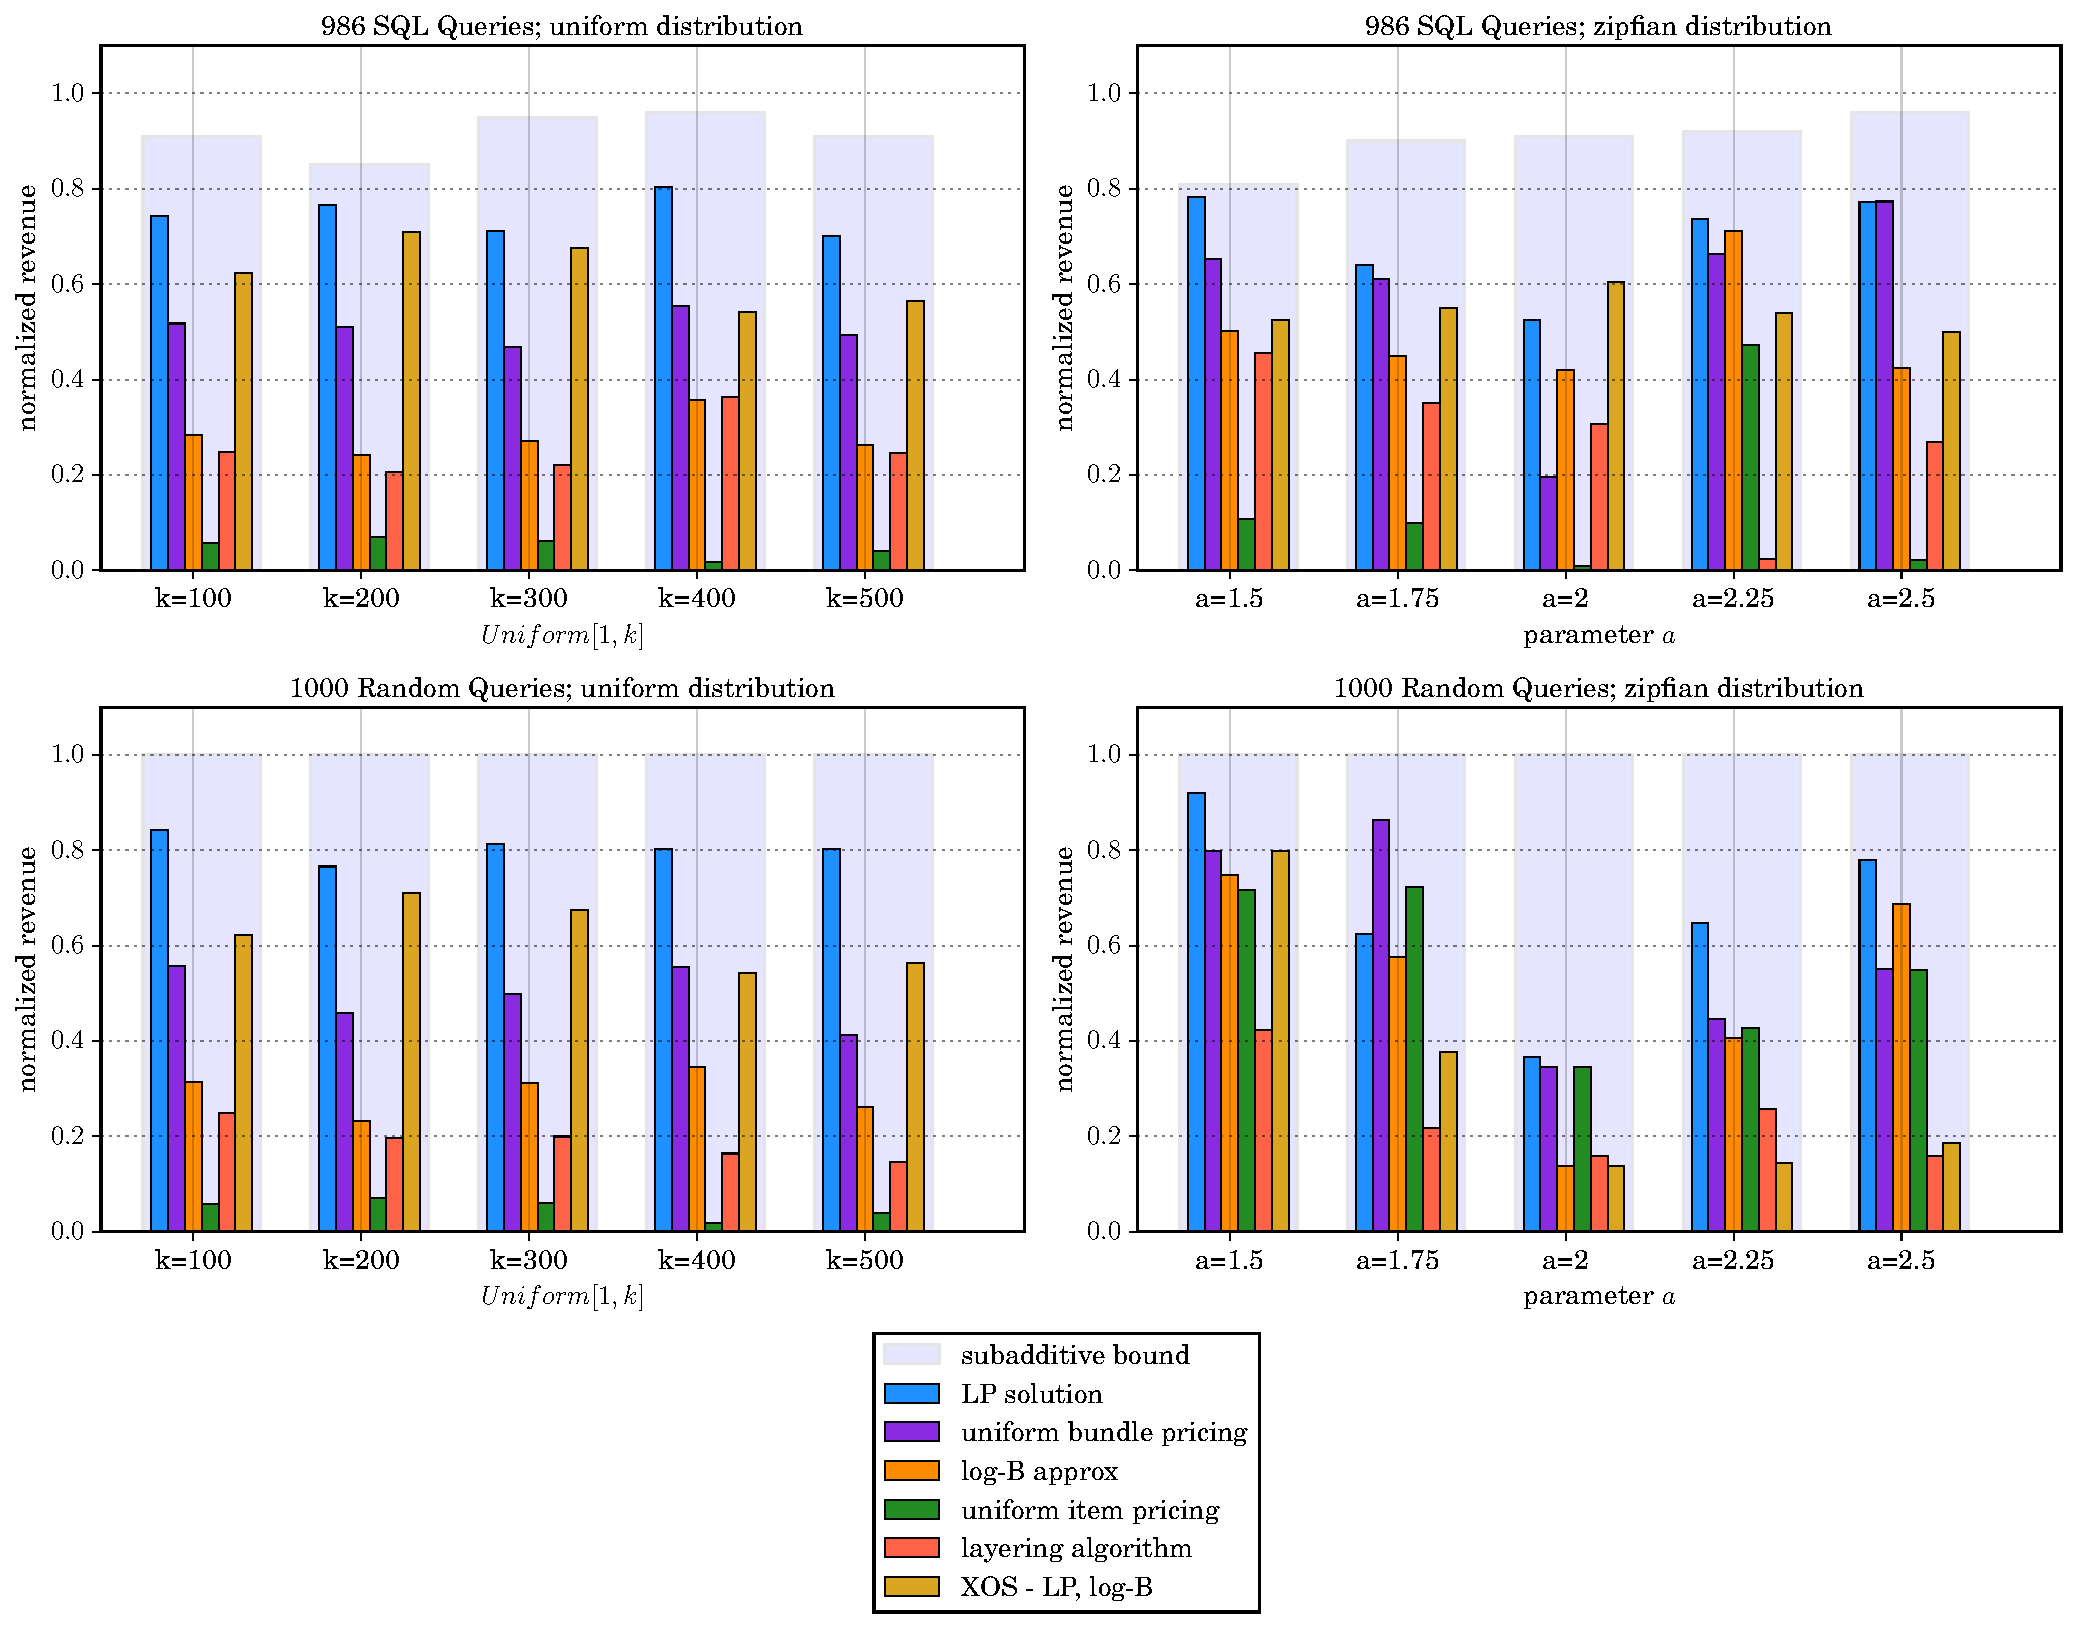
\includegraphics[scale=0.40]{uniformzipfianvaluations.pdf}
	\caption{Sampling Bundle Valuations: SQL workload and random workload} \label{fig:unifzipfian}
\end{figure}  

\smallskip
\introparagraph{Sampling from uniform distribution} The first experiment samples valuations from the uniform distribution. Figure~\ref{fig:unifzipfian} shows the performance of all algorithms. Since the valuations for bundles are relatively close to each other, item pricing struggles to generate good prices. As we will see later, when the size of the bundle is correlated with the bundle valuation, item pricing will perform very well.  We also perform the experiment with zipfian distribution. \lpip is again better than other algorithms and \ubp is close to \lpip. Not surprisingly, the layering algorithm does not perform well except in the case of zipfian distribution with exponent smaller than $2$. Indeed, for $a < 2$, zipfian distribution assigns a large valuation to some hyperedge that contributes significantly to the total revenue. In such cases, the layering algorithm can always extract full revenue from the layer containing high valuation edges and perform well in practice. As the zipfian exponent becomes greater than two, the spread of valuations becomes smaller and layering algorithm becomes worse. The same behavior is also observed for the exponential distribution. 

\subsubsection{Scaling Bundle Valuations} So far, the valuations are sampled independently of the edge size. Our next experiment will correlate the size of the edge with the valuation that is assigned to it. To this end, we will sample valuation from parameterized exponential and normal distribution as follows: we assign $v_e \sim {\rm exponential}(\beta = m^k)$ where $\beta$ is the mean of the distribution. Similarly, for normal distribution, $v_e \sim \mathcal{N}(\mu = m^k,\, \sigma^2 = 10)$. Here $k$ is the parameter that we will vary. Figure~\ref{fig:scalingedge} shows the result for different values of the parameter $k$. For both distributions, when $k \geq 1$, most of the revenue is concentrated in a few edges that have extremely large valuations. In this situation, \lpip and \ubp perform well. We also investigate how XOS pricing functions behave. To define the function, we take the maximum over the best pricing vector generated by the item pricing algorithms. Not surprisingly, this does not give good results in our experiments. The last observation is to notice the approximation of \uip. The optimization of relaxing the uniform item prices via  LP dramatically increases the revenue extracted (sometimes by as much as 5x).

\begin{figure}[!t]
	\centering
	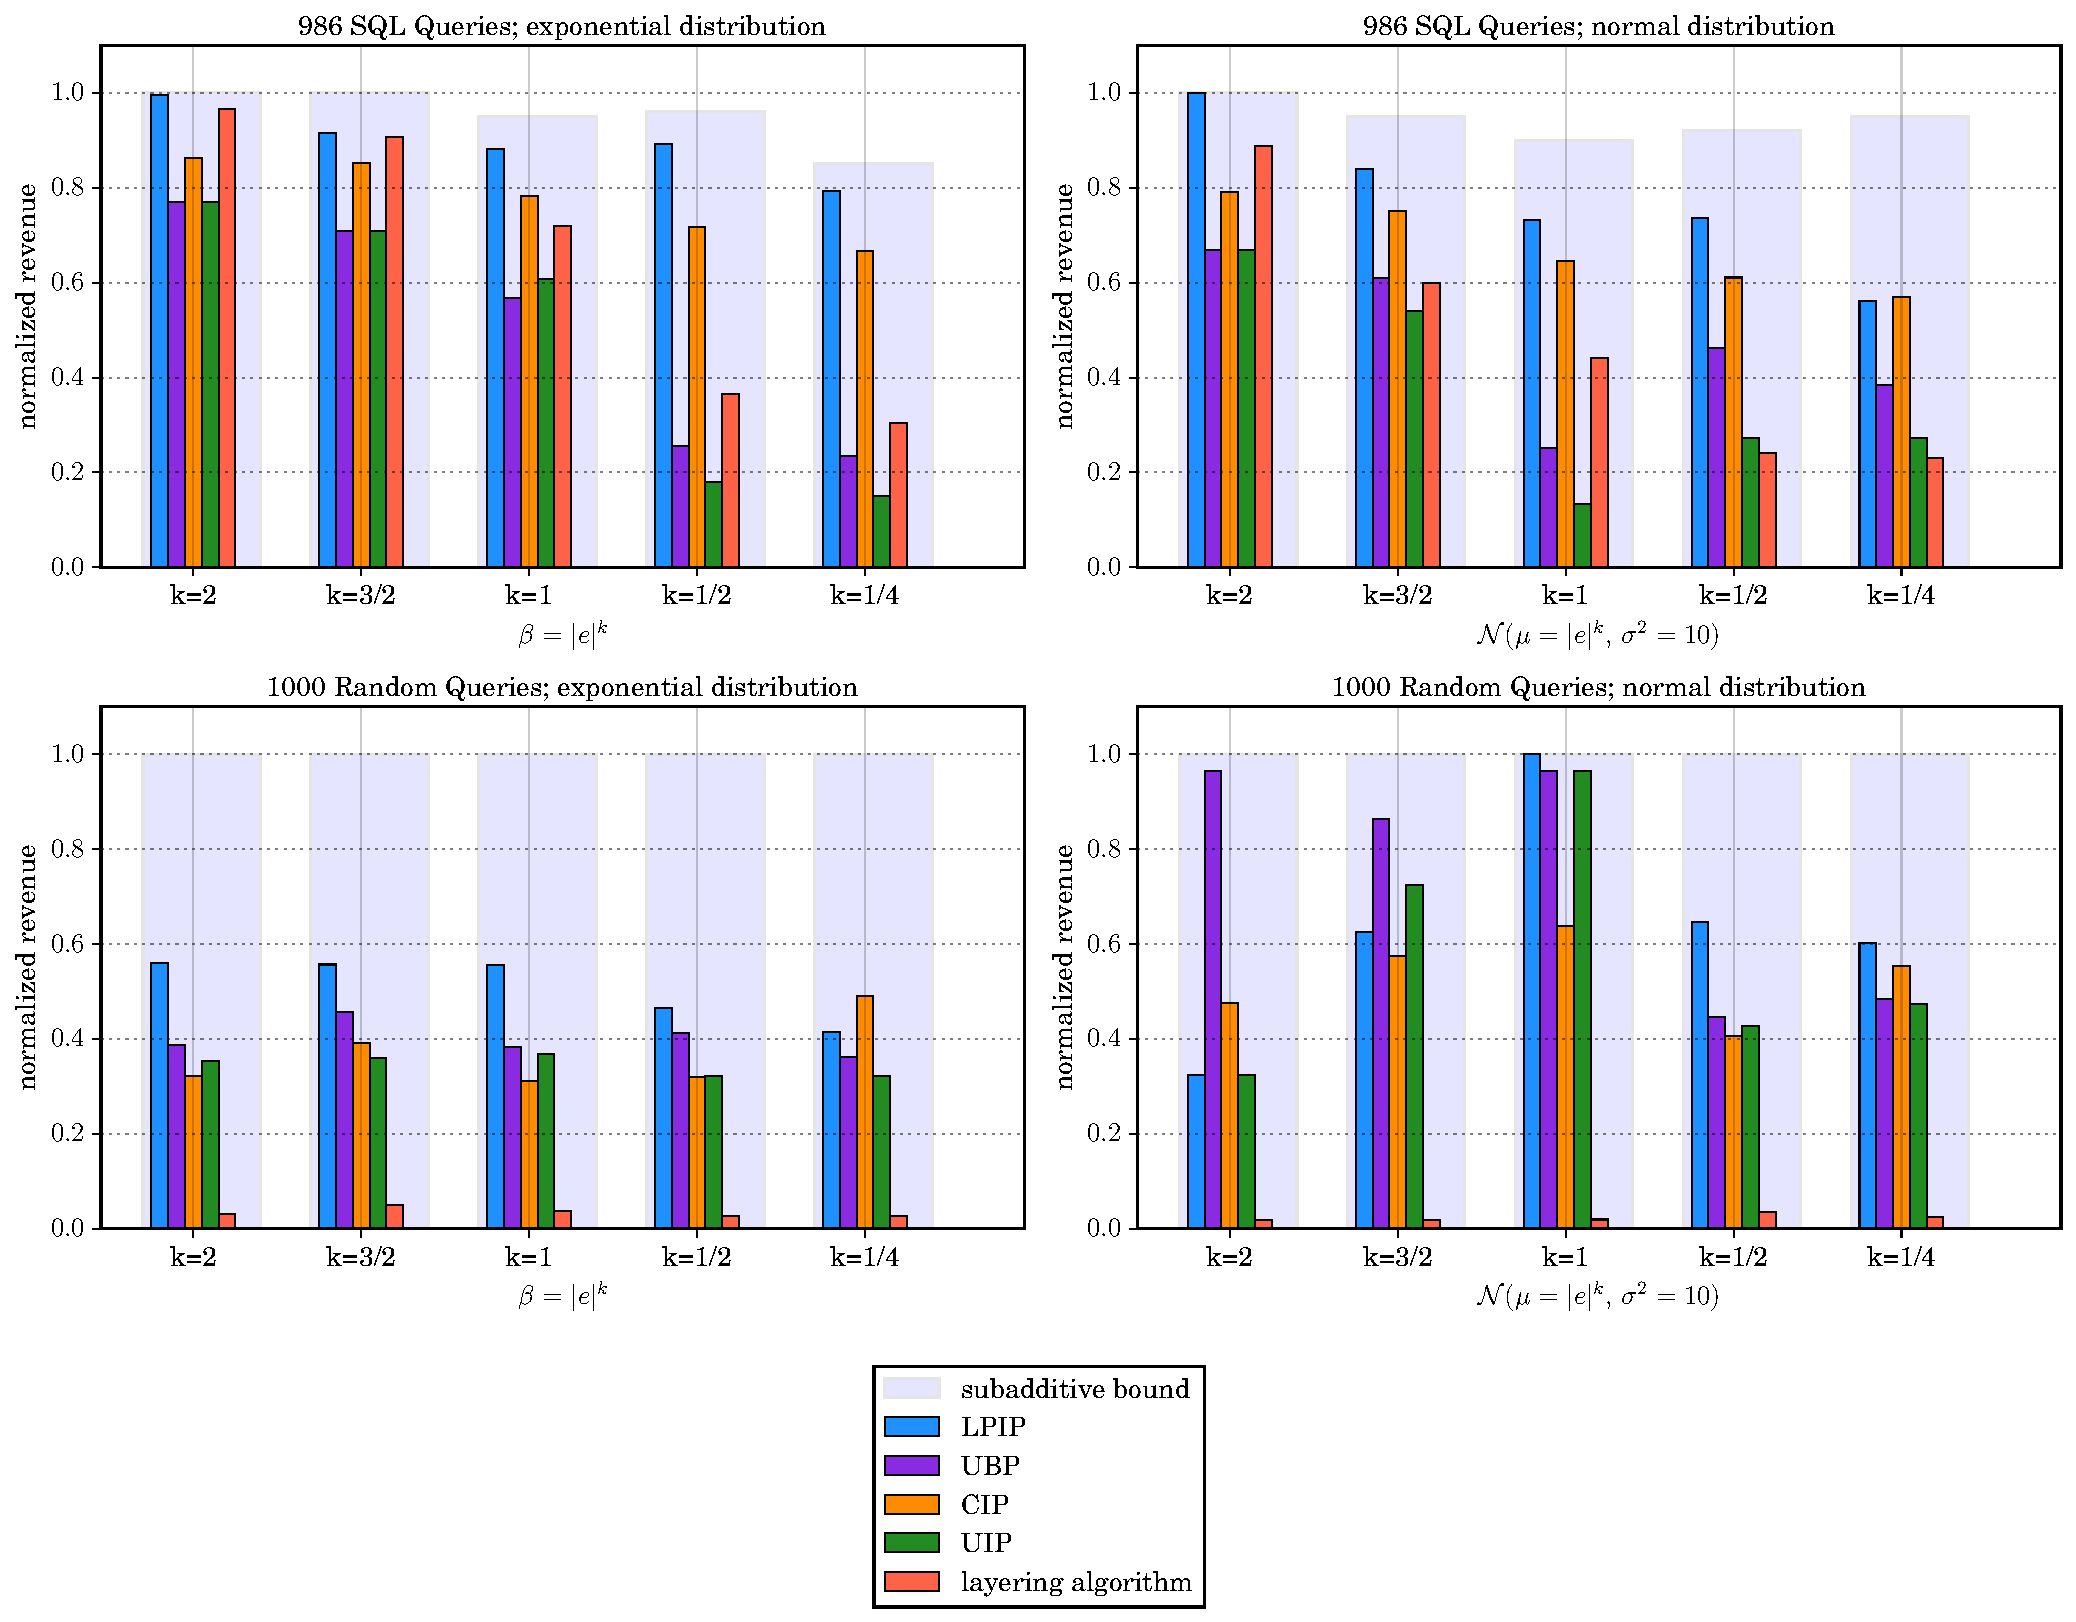
\includegraphics[scale=0.40]{queriesscalingedgesize.pdf}
	\caption{Scaling Bundle Valuations: SQL workload and random workload} \label{fig:scalingedge}
\end{figure}  

\subsubsection{Sampling Item Prices} The last of set of experiments on the SQL workload is to understand the behavior of algorithms when the valuation of edges is defined by an \emph{additive model}. More specifically, we define $k$ different distributions $\{D_i\}_{i=1}^{k}$ from which items will draw their prices and a special distribution $\tilde{D}$ which will assign each item which distribution it will sample from. The valuation of an edge is the defined as $v_e = \sum_{j \in e} x_j \sim D_{\ell_j}$ where $\ell_j \sim \tilde{D}$. Intuitively, this model will capture the scenario where parts of the database have non-uniform value and some parts are much more valuable than others. To see why this setting can be practical interest, consider a research analyst in banking who gives stock recommendations. While public information about companies and stocks may be cheap, the research analysts buy and sell recommendations will be of much higher value. For the purpose of experiments, we fix $D_i$ to $\textsf{Uniform}[i, i+1]$ and set $\tilde{D}$ to $\textsf{Uniform}[1, k]$ or $\textsf{Binomial}(k, 1/2)$ while varying $k$. Figure~\ref{fig:mixing} shows the results of this experiment. Here, \lpip outperforms all other algorithms. For smaller values of $k$, the valuation of edges are close to $|e|$. In this case, there is no gap between uniform item pricing and its LP variant. As  the value of $k$ increases, uniform item pricing does slightly worse than \lpip.


\begin{figure}[!t]
	\centering
	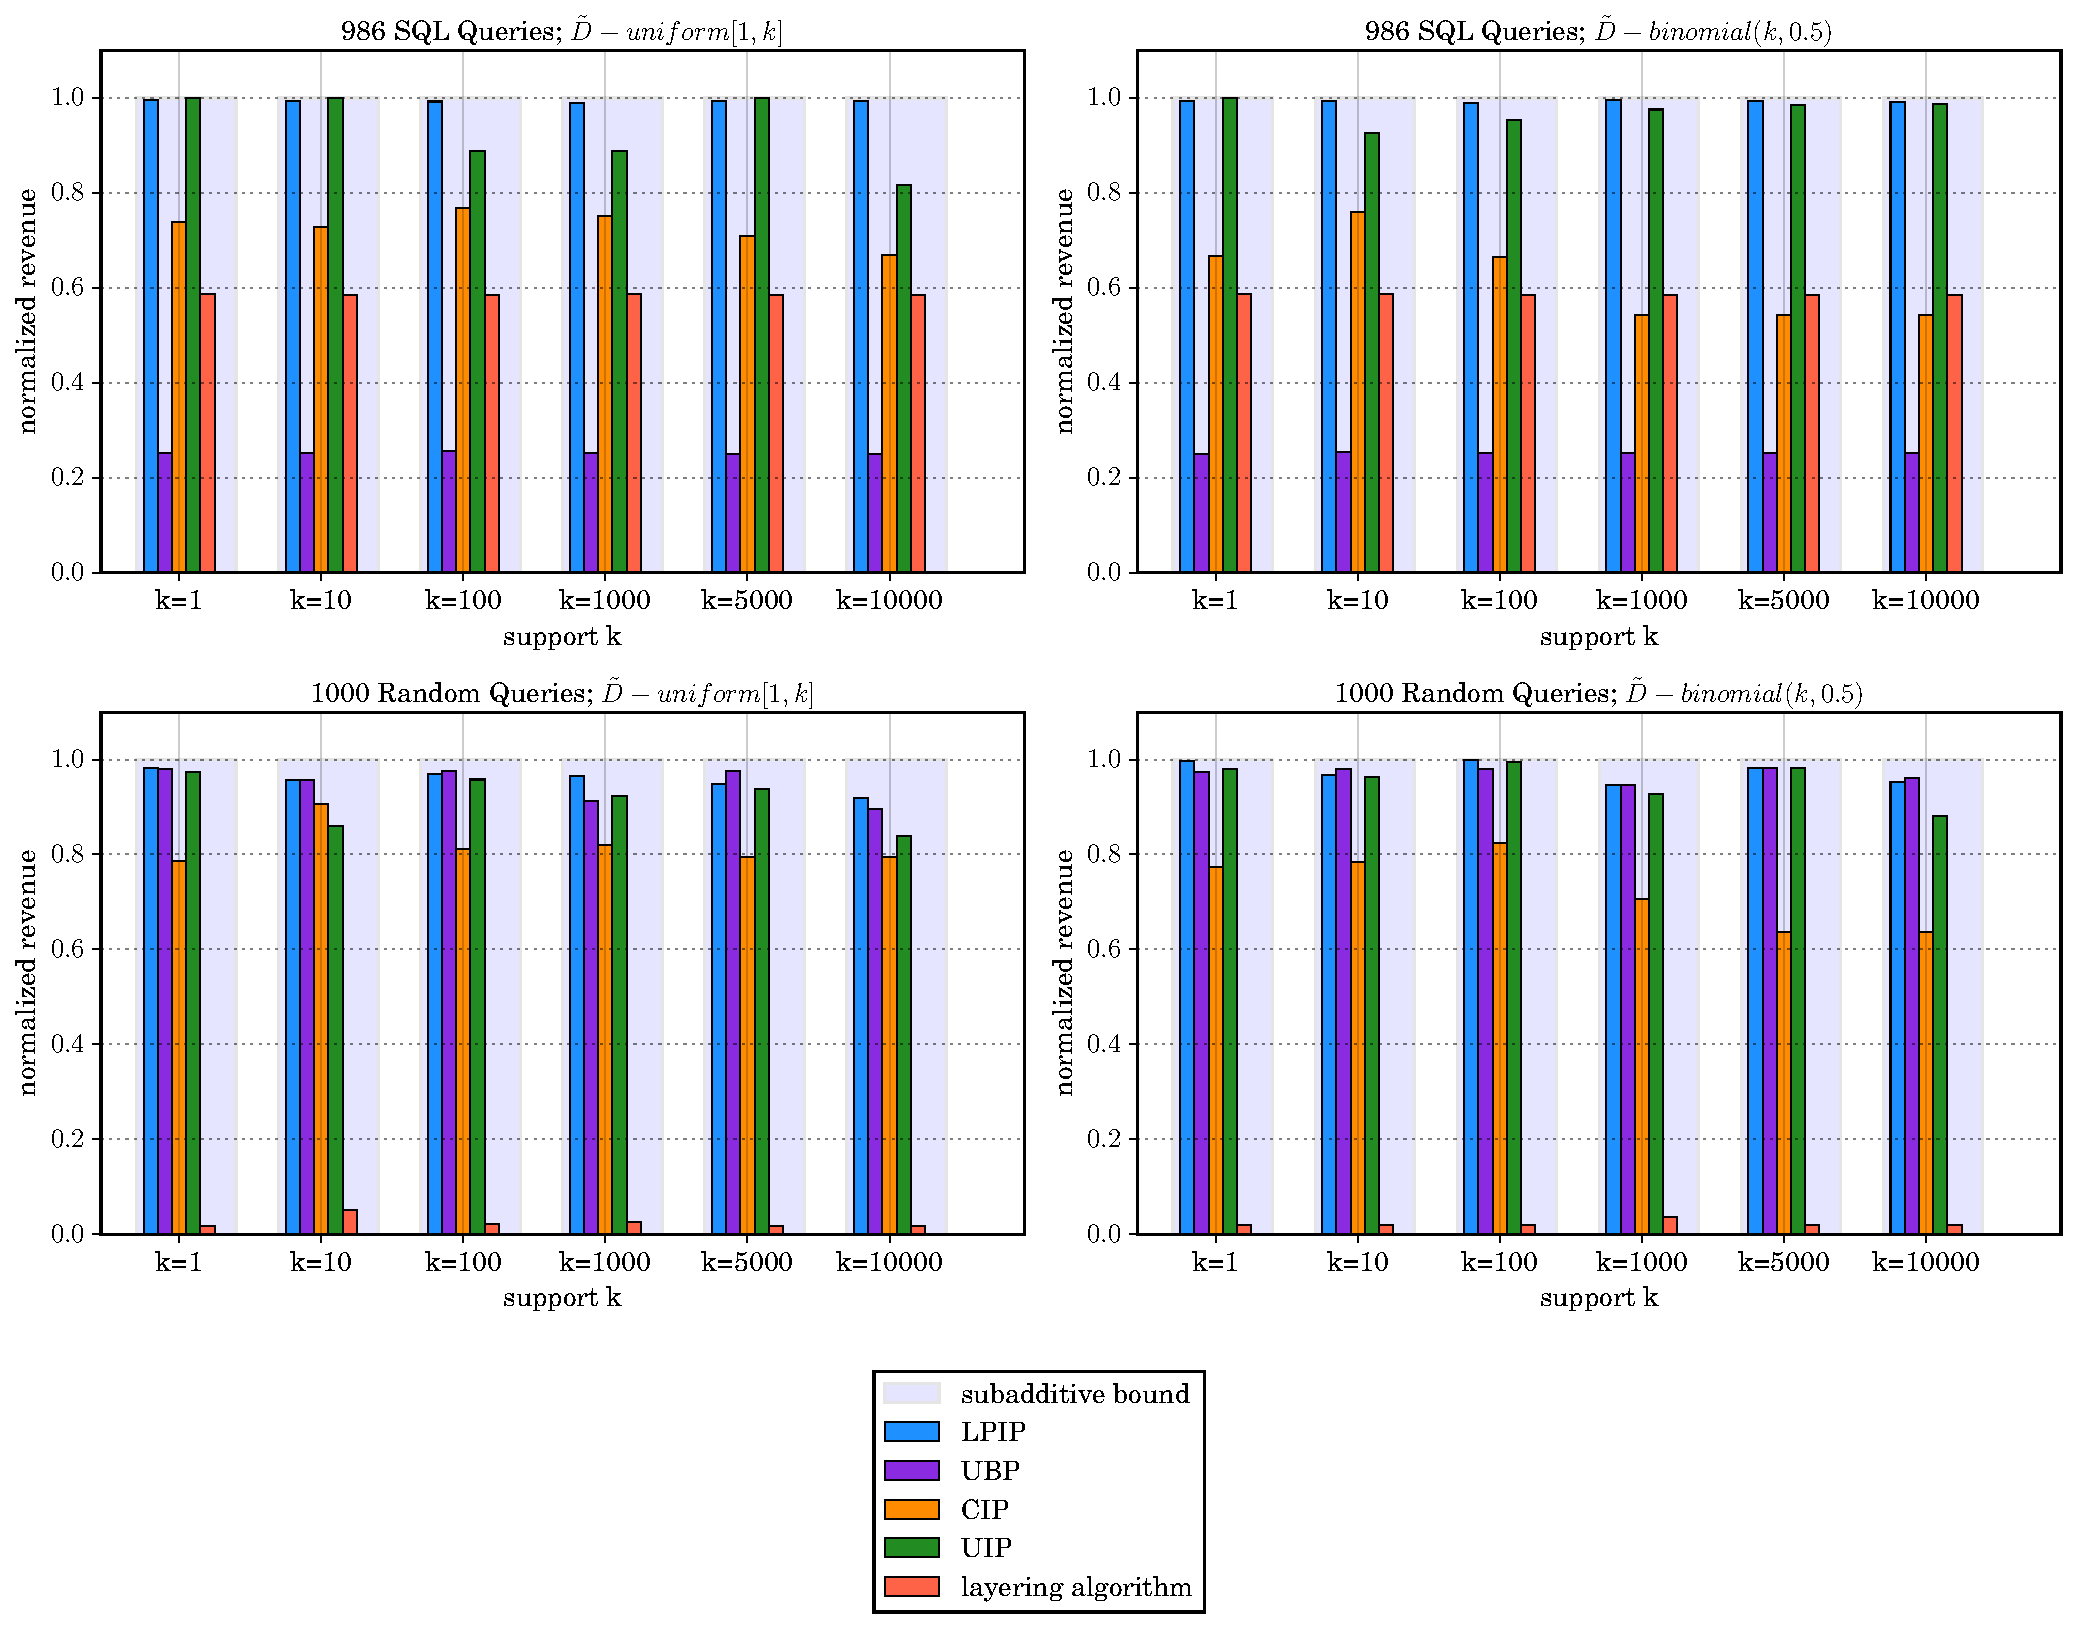
\includegraphics[scale=0.40]{queriesmixing.pdf}
	\caption{Sampling Item Prices: SQL workload and random workload} \label{fig:mixing}
\end{figure}  

\subsection{Experiment Results for Random Query Workload}


The second half of our experiments focuses on random query workload. For the following experiments, we generate $1000$ random queries and fix the resulting hypergraph. 

\subsubsection{Sampling Bundle Valuations}

In this experiment, valuations for each edge is chosen from the uniform distribution. Once again, uniform bundle pricing outperforms other approximation algorithms. Because of the high degree of overlap between hyperedges, the layering algorithm does not perform well as the number of levels formed is fairly large and thus, the algorithm cannot pack too many edges at any level.

\subsubsection{Scaling Bundle Valuations} In this valuation model, for random hypergraphs, uniform bundle pricing and \lpip are the best performing. The \cip algorithm does not perform well even though it is theoretically optimal. This is because going over all capacity vectors with limited supply is extremely expensive. In our implementation, running the linear program for a large number of capacity vectors takes close to $2$ hours in total (we discuss reasons for this in the next section). Thus, we reduce the number of capacity vectors that we try by increasing the $(1+\epsilon)$ parameter. This introduces a factor of $(1+\epsilon)$ in the approximation ratio but allows for the running time to be smaller. This step improves the approximation factor of \cip (and in some cases, outperforms \lpip) but remains marginally inferior to \lpip . Note that this issue is observed to a lesser extent in the SQL workload since the largest degree item is shared by $22$ edges but random hypergraph has the largest degree close to $400$. The second row in Figure~\ref{fig:scalingedge} shows the results for random query workload. For the exponential distribution, no algorithm is close to optimal. We believe this is not an anomaly but rather the subaddtive bound not being as good as it should be.

\subsubsection{Sampling Item Prices} For this setting, all algorithms give a good approximation ratio except the layering algorithm. Bottom row in figure~\ref*{fig:mixing} shows the experimental results for random queries. Since the size of the edges is relatively concentrated, uniform item pricing and uniform bundle pricing do very well. Although \lpip does the best, it does not improve by much since uniform item pricing gives a good baseline solution.  Once again, the layering algorithm is the worst performing out of all.


\subsection{Running Time of Algorithms}

\begin{table*}[] \centering
	%\ra{1.3}
	\begin{small}
		\begin{tabular}{@{}lrrrrr@{}}\toprule
			\textbf{Workload} & \textbf{LP} & \textbf{Uniform Bundle Pricing} & \textbf{Uniform Item Pricing} & $\mathbf{O(\log B)}$ & \textbf{Layering}  \\ \midrule
			
			\textbf{SQL Queries} &  60.62 & 15.50 & 25.45 & 812.67 & 15.67 \\ \hdashline
			\textbf{Random Queries} &  95.81 & 18.68 &  29.82 &1800 & 50.19 \\
			\bottomrule
		\end{tabular}
	\end{small}
	\caption{Algorithm running times (in seconds) for different workloads}
	\label{table:runtime}
\end{table*}

In this section we discuss the running time of the algorithms. Table~\ref{table:runtime} shows the run time of all algorithms for both the workloads. The most time efficient algorithms are uniform bundle pricing, uniform item pricing and the layering algorithm. Uniform bundle pricing and uniform item pricing depend only on number of hyperedges and the number of items in the hypergraph. Thus, they are very fast to run in practice. Layering algorithm is slightly slower but comparable in performance. Note that layering is faster on SQL workload as compared to the random hypergraphs since the maximum degree is much smaller. The two slowest running algorithms are \lpip and \cip as they require running multiple linear programs. In practice, \lpip is faster than \cip. This is because of the size of the linear program is very different. Observe that in our setting number of edges $m \sim 1000$ is much smaller than the number of items $n = 15000$. \lpip  has one constraint per bundle (thus, at most $m$ constraints) but \cip has one contraint per item ($n$ constraints in total). This dramatically influences the running time of the two algorithms. \cip uses $(1+\epsilon)$ as a parameter where $\epsilon$ controls the limited supply available for each item. We adjust the value of $\epsilon$ for both workloads to ensure that the running time is at most $30$ minutes. We fix $\epsilon = 0.2$ for SQL workload and $\epsilon = 4$ for random workload based on our empirical observations.

\section{Conclusion}
\label{sec:conclusion}

In this paper, we study the problem of revenue maximization in the context of query-based pricing.
We cast the task as a bundle pricing problem for single-minded buyers and unlimited supply, and then
perform a detailed experimental evaluation on the effectiveness of various approximation
algorithms that provide different worst-case approximation guarantees. Our results show that the specific
bundle structure often means that simple item-pricing algorithms perform much better than their worst-case
guarantees.  

There are several open questions that remain. First, is it possible to 
come up with algorithms and approximation analyses that are beyond worst-case, and take into account
the structure of either the bundles, or the valuations? Further, can we design 
algorithms that directly construct XOS pricing functions that can perform better than either item pricing
or uniform bundle pricing?



% Bibliography
\bibliographystyle{ACM-Reference-Format}
\bibliography{qpricing,reference}

\end{document}

